\documentclass[12pt, a4paper]{article}

% -----------------------------------------------------------------------
% Packages
% -----------------------------------------------------------------------
\usepackage[utf8]{inputenc}
\usepackage[T1]{fontenc}
\usepackage{amsmath, amssymb, amsthm}
\usepackage{geometry}
\usepackage{hyperref}
\usepackage{graphicx}
\usepackage{booktabs}
\usepackage{array}
\usepackage{enumitem}
\usepackage{cite}
\usepackage{listings}
\usepackage{xcolor}
\usepackage{caption}
\usepackage{float}
\usepackage{tikz}
\usetikzlibrary{positioning}

\geometry{margin=1in}

% -----------------------------------------------------------------------
% Theorem Environments
% -----------------------------------------------------------------------
\newtheorem{theorem}{Theorem}[section]
\newtheorem{proposition}[theorem]{Proposition}
\newtheorem{corollary}[theorem]{Corollary}
\newtheorem{lemma}[theorem]{Lemma}
\theoremstyle{definition}
\newtheorem{definition}[theorem]{Definition}
\newtheorem{example}[theorem]{Example}
\newtheorem{assumption}{Assumption}
\theoremstyle{remark}
\newtheorem{remark}[theorem]{Remark}

% -----------------------------------------------------------------------
% Code Listing Style
% -----------------------------------------------------------------------
\lstset{
    language=Python,
    basicstyle=\ttfamily\small,
    keywordstyle=\color{blue},
    commentstyle=\color{gray},
    stringstyle=\color{orange!80!black},
    showstringspaces=false,
    frame=single,
    rulecolor=\color{lightgray},
    breaklines=true,
    numbers=left,
    numberstyle=\tiny\color{gray},
    numbersep=5pt,
}

% -----------------------------------------------------------------------
% Title
% -----------------------------------------------------------------------
\title{
    \textbf{OS Synchronization as Symmetry Restrictions in $S_n$} \\
    \large A Computational and Struct\textbfural Study
}
\author{Om Pranab Mohanty}
\date{2026}

% -----------------------------------------------------------------------
\begin{document}
% -----------------------------------------------------------------------

\maketitle

\begin{abstract}
Classical operating system synchronization mechanisms --- mutual exclusion,
round-robin scheduling, and deadlock --- are typically described in operational
terms: semaphores, locks, and wait queues. This paper proposes a complementary
structural description using elementary group theory. We model the space of all
process schedules for a single scheduling epoch as the symmetric group $S_n$,
where each permutation represents a total ordering of $n$ concurrent processes
under the assumptions of exactly one execution slot per epoch, no preemption,
and no priority.

We show that three synchronization constraints correspond to well-known
algebraic substructures: mutual exclusion corresponds to a stabilizer subgroup
$M(x) = \mathrm{Stab}_{S_n}(x) \leq S_n$ of order $(n-1)!$; round-robin
scheduling corresponds to a cyclic subgroup $\langle c \rangle \cong
\mathbb{Z}_n$ of order $n$; and deadlock, under an explicit modeling
assumption, corresponds to the identity element $e \in S_n$.

The subgroups $M(x)$ and $\langle c \rangle$ are incomparable for $n \geq 3$,
with $M(x) \cap \langle c \rangle = \{e\}$, reflecting a structural separation
between safety and fairness constraints in the scheduling space. These
correspondences are verified computationally in Python for
$n \in \{2,3,4,5,6\}$ using only first-principles implementations with no
computer algebra library. Source code and notebooks are available at
\cite{repo}.
\end{abstract}

\tableofcontents
\newpage

% -----------------------------------------------------------------------
\section{Introduction}
% -----------------------------------------------------------------------

Operating systems manage concurrent processes through synchronization
primitives. These primitives are well understood operationally: a mutex
prevents two processes from entering a critical section simultaneously; a
round-robin scheduler grants each process a fair time quantum in cyclic
order; a deadlock is a state in which a circular chain of waiting processes
prevents any forward progress. Standard references describe these mechanisms
through algorithms, pseudocode, and state diagrams \cite{silberschatz}.

What is less often examined is whether these mechanisms admit a common
\emph{structural} description. This paper explores one such description,
grounded in the theory of permutation groups \cite{gallian}.

If we have $n$ concurrent processes, any total ordering of those processes
is a bijection from the process set to itself --- a permutation. The set
of all such orderings forms the symmetric group $S_n$. Synchronization
constraints restrict which orderings are admissible. We show that for three
classical constraints, the admissible sets are subgroups of $S_n$ with
recognizable algebraic structure.

It is important to note that not every synchronization constraint defines a
subgroup of $S_n$. We focus specifically on those constraints whose
admissible sets are closed under composition and inverse. This closure
property is not assumed; it is verified formally and computationally for
each constraint.

\subsection*{Contribution}

The novelty of this work lies not in new mathematical results --- the
correspondences follow directly from standard definitions in group theory ---
but in explicitly unifying three OS synchronization primitives within a
single subgroup-theoretic framework and providing an executable, transparent
computational verification of the structural picture. The accompanied source
code \cite{repo} implements all structures from first principles.

\subsection*{AI Tools Used}

This project used Claude (Anthropic) \cite{claude} as an AI assistant
during development. Claude was used to assist in writing Python source
code, generating Jupyter notebook structure, and drafting this manuscript.
All mathematical content, claims, proofs, and interpretations were reviewed,
understood, and verified by the author. Computational outputs were
independently executed and checked. AI assistance is disclosed in
accordance with academic integrity requirements.

\subsection*{Scope}

This is a formalization and verification project. The model covers total
orderings within a single scheduling epoch and does not capture preemption,
priority scheduling, or partial orders. The deadlock claim relies on an
explicit modeling assumption stated in Section~\ref{sec:deadlock}. No new
results in either group theory or operating systems are claimed.

% -----------------------------------------------------------------------
\section{Model Assumptions}
\label{sec:assumptions}
% -----------------------------------------------------------------------

All claims in Sections~\ref{sec:claim1}--\ref{sec:deadlock} are made
within the following explicitly stated modeling boundary.

\begin{assumption}[Finite Process Set]
\label{ass:finite}
The system contains exactly $n \geq 2$ distinguishable processes,
labelled $1, 2, \ldots, n$. We write $P = \{1, \ldots, n\}$.
\end{assumption}

\begin{assumption}[Single Scheduling Epoch]
\label{ass:epoch}
A schedule represents a single epoch of execution --- a complete assignment
of all $n$ processes to $n$ execution slots at one point in time. The model
does not capture dynamic time evolution, preemption, context switching
between epochs, or multi-step scheduling histories.
\end{assumption}

\begin{assumption}[Total Ordering]
\label{ass:total}
Each epoch assigns each process exactly one execution slot, and each slot
is assigned to exactly one process. A schedule is therefore a bijection on
$P$: no two processes share a slot, and no process is unscheduled.
\end{assumption}

\begin{assumption}[No Preemption Within an Epoch]
\label{ass:nopreempt}
Once an epoch's schedule is fixed, it executes to completion without
interruption or rescheduling.
\end{assumption}

\begin{assumption}[No Priority or Probabilistic Weighting]
\label{ass:nopriority}
All processes are treated as equally schedulable. The model contains no
weights, priority levels, or probability distributions over schedules.
\end{assumption}

\begin{assumption}[Single Critical Slot]
\label{ass:slot}
The mutual exclusion constraint is modelled with respect to a single
designated slot $x \in P$. Generalisation to multi-resource mutex via
intersections of stabilizers is noted in Section~\ref{sec:extensions}
but not developed here.
\end{assumption}

% -----------------------------------------------------------------------
\section{Background}
% -----------------------------------------------------------------------

\subsection{Symmetric Groups}

We recall the necessary definitions. The primary algebraic reference is
Gallian \cite{gallian}.

\begin{definition}[Symmetric Group]
Let $P = \{1, 2, \ldots, n\}$. The \emph{symmetric group} $S_n$ is the
set of all bijections $\sigma: P \to P$, equipped with function composition:
\[
(\sigma \circ \tau)(i) = \sigma(\tau(i)), \quad i \in P.
\]
\end{definition}

\begin{proposition}
$(S_n, \circ)$ is a group of order $|S_n| = n!$
\end{proposition}

\begin{definition}[Subgroup]
A non-empty subset $H \subseteq S_n$ is a \emph{subgroup}, written
$H \leq S_n$, if it contains the identity element, is closed under
composition, and is closed under inverses.
\end{definition}

\begin{theorem}[Lagrange \cite{gallian}]
If $H \leq S_n$, then $|H|$ divides $|S_n| = n!$
\end{theorem}

\begin{definition}[Group Action, Orbit, Stabilizer]
The natural \emph{action} of $S_n$ on $P$ is $(\sigma, i) \mapsto \sigma(i)$.
For $x \in P$:
\[
\mathrm{Orb}(x) = \{\sigma(x) \mid \sigma \in S_n\}, \qquad
\mathrm{Stab}(x) = \{\sigma \in S_n \mid \sigma(x) = x\}.
\]
\end{definition}

\begin{theorem}[Orbit-Stabilizer \cite{gallian}]
\label{thm:orbit-stab}
For any $x \in P$:
$|S_n| = |\mathrm{Orb}(x)| \cdot |\mathrm{Stab}(x)|$.
\end{theorem}

\subsection{Cycles and Cyclic Subgroups}

\begin{definition}[Cycle Notation]
The permutation $(a_1\ a_2\ \cdots\ a_k)$ maps $a_1 \mapsto a_2 \mapsto
\cdots \mapsto a_k \mapsto a_1$ and fixes all other elements. Such a
permutation is called a \emph{$k$-cycle}.
\end{definition}

\begin{definition}[Cyclic Subgroup]
For $\sigma \in S_n$, the \emph{cyclic subgroup} generated by $\sigma$ is
$\langle \sigma \rangle = \{\sigma^k \mid k \in \mathbb{Z}\}$, where
$\sigma^0 = e$.
\end{definition}

\begin{lemma}[Order of an $n$-Cycle]
\label{lem:ncycle}
Any $n$-cycle in $S_n$ has order $n$.
\end{lemma}

\begin{proof}
Let $c = (a_1\ a_2\ \cdots\ a_n)$. Then $c^k(a_1) = a_{1+k \bmod n}$.
For $c^k = e$ we need $1 + k \equiv 1 \pmod{n}$, i.e.\ $n \mid k$.
The smallest positive such $k$ is $n$, so $\mathrm{ord}(c) = n$.
\end{proof}

% -----------------------------------------------------------------------
\section{Formal Model}
% -----------------------------------------------------------------------

\begin{definition}[Schedule]
Under Assumptions~\ref{ass:finite}--\ref{ass:total}, a \emph{schedule}
is a bijection $\sigma: P \to P$. If $\sigma(i) = k$, process $i$ is
assigned to execution slot $k$ in the current epoch.
\end{definition}

\begin{remark}
A schedule is a static assignment for one epoch. It does not model the
dynamic process by which schedules are selected over time, nor properties
such as liveness or starvation across multiple epochs.
\end{remark}

\begin{definition}[Scheduling Space]
The \emph{unrestricted scheduling space} is $S_n$ --- the set of all
schedules admitted by Assumptions~\ref{ass:finite}--\ref{ass:total}.
\end{definition}

\begin{definition}[Synchronization Constraint]
\label{def:constraint}
A \emph{synchronization constraint} is a predicate $C: S_n \to \{0,1\}$.
The \emph{admissible set} is
$\mathcal{A}_C = \{\sigma \in S_n \mid C(\sigma) = 1\}$.
\end{definition}

\begin{remark}[Subgroup Requirement]
\label{rem:subgroup}
Not every synchronization constraint produces a subgroup. For each
constraint studied here, we verify explicitly that $\mathcal{A}_C$ is
closed under composition, closed under inverses, and contains the identity.
This makes $\mathcal{A}_C \leq S_n$. Closure is proved in each case, not
assumed.
\end{remark}

% -----------------------------------------------------------------------
\section{Claim 1: The Scheduling Space is $S_n$}
\label{sec:claim1}
% -----------------------------------------------------------------------

\begin{proposition}
The unrestricted scheduling space has order $|S_n| = n!$
\end{proposition}

\begin{proof}
A bijection from $P$ to $P$ is determined by assigning images to
$1, 2, \ldots, n$ sequentially: $n$ choices for $\sigma(1)$, $n-1$ for
$\sigma(2)$, and so on. The total is $n \cdot (n-1) \cdots 1 = n!$.
\end{proof}

\begin{table}[H]
\centering
\begin{tabular}{@{}ccc@{}}
\toprule
$n$ & $|S_n|$ & $n!$ \\
\midrule
2 & 2   & 2   \\
3 & 6   & 6   \\
4 & 24  & 24  \\
5 & 120 & 120 \\
6 & 720 & 720 \\
\bottomrule
\end{tabular}
\caption{Size of the scheduling space $S_n$, verified computationally.}
\label{tab:sn}
\end{table}

% -----------------------------------------------------------------------
\section{Claim 2: Mutual Exclusion as a Stabilizer Subgroup}
\label{sec:mutex}
% -----------------------------------------------------------------------

\subsection{The Mutex Constraint}

We model the critical section as a designated slot $x \in P$ under
Assumption~\ref{ass:slot}. A schedule respects mutual exclusion if the
process assigned to slot $x$ is not displaced:

\begin{definition}[Mutex-Admissible Schedule]
$\sigma \in S_n$ is \emph{mutex-admissible} with respect to slot
$x \in P$ if $\sigma(x) = x$.
\end{definition}

\begin{theorem}
\label{thm:mutex}
Let $M(x) = \{\sigma \in S_n \mid \sigma(x) = x\}$. Then:
\begin{enumerate}[(i)]
    \item $M(x) = \mathrm{Stab}_{S_n}(x)$ is a subgroup of $S_n$.
    \item $|M(x)| = (n-1)!$
    \item $M(x) \cong S_{n-1}$.
    \item The index $[S_n : M(x)] = n$.
\end{enumerate}
\end{theorem}

\begin{proof}
\textit{(i) Subgroup.}
$e(x) = x$, so $e \in M(x)$.
For $\sigma, \tau \in M(x)$:
$(\sigma \circ \tau)(x) = \sigma(\tau(x)) = \sigma(x) = x$,
so $M(x)$ is closed under composition.
If $\sigma(x) = x$, applying $\sigma^{-1}$ gives $x = \sigma^{-1}(x)$,
so $M(x)$ is closed under inverses. Hence $M(x) \leq S_n$.

\textit{(ii) Order.}
The orbit of any $x \in P$ under $S_n$ is all of $P$
(for any $y \in P$, there exists $\sigma$ mapping $x$ to $y$), so
$|\mathrm{Orb}(x)| = n$. By Theorem~\ref{thm:orbit-stab}:
$n! = n \cdot |M(x)|$, giving $|M(x)| = (n-1)!$

\textit{(iii) Isomorphism.}
Any $\sigma \in M(x)$ fixes $x$ and acts freely on $P \setminus \{x\}$.
The restriction map $\sigma \mapsto \sigma|_{P \setminus \{x\}}$ is a
group isomorphism $M(x) \to S_{n-1}$.

\textit{(iv) Index.} $[S_n : M(x)] = n! / (n-1)! = n$.
\end{proof}

\subsection{Coset Decomposition}

The $n$ cosets of $M(x)$ in $S_n$ partition the scheduling space. The
identity coset $M(x)$ contains all admissible schedules. Each of the
remaining $n-1$ cosets corresponds to a distinct process illegally
occupying slot $x$:
\[
S_n = M(x) \;\cup\; \sigma_1 M(x) \;\cup\; \cdots \;\cup\;
\sigma_{n-1}M(x).
\]

\begin{table}[H]
\centering
\begin{tabular}{@{}cccccc@{}}
\toprule
$n$ & $|S_n|$ & $|M(x)|$ & $(n-1)!$ & Index & Subgroup \\
\midrule
2 & 2   & 1   & 1   & 2 & \checkmark \\
3 & 6   & 2   & 2   & 3 & \checkmark \\
4 & 24  & 6   & 6   & 4 & \checkmark \\
5 & 120 & 24  & 24  & 5 & \checkmark \\
6 & 720 & 120 & 120 & 6 & \checkmark \\
\bottomrule
\end{tabular}
\caption{Stabilizer subgroup orders, verified computationally.}
\label{tab:stab}
\end{table}

% -----------------------------------------------------------------------
\section{Claim 3: Round-Robin as a Cyclic Subgroup}
\label{sec:rr}
% -----------------------------------------------------------------------

\begin{definition}[Round-Robin Permutation]
The \emph{round-robin permutation} is the $n$-cycle:
\[
c = (1\ 2\ 3\ \cdots\ n), \qquad
c(i) = \begin{cases} i+1 & i < n, \\ 1 & i = n. \end{cases}
\]
\end{definition}

\begin{theorem}
\label{thm:rr}
The cyclic subgroup $\langle c \rangle \leq S_n$ satisfies:
\begin{enumerate}[(i)]
    \item $|\langle c \rangle| = n$.
    \item $\langle c \rangle \cong \mathbb{Z}_n$.
    \item $\langle c \rangle$ acts transitively on $P$.
    \item $\langle c \rangle$ is abelian.
    \item $\langle c \rangle$ is not normal in $S_n$ for $n \geq 3$.
\end{enumerate}
\end{theorem}

\begin{proof}
\textit{(i)} By Lemma~\ref{lem:ncycle}, $\mathrm{ord}(c) = n$,
so $|\langle c \rangle| = n$.

\textit{(ii)} The map $\varphi: \mathbb{Z}_n \to \langle c \rangle$,
$\varphi(k) = c^k$, is a bijective homomorphism:
$\varphi(j + k \bmod n) = c^{j+k} = c^j \circ c^k = \varphi(j) \circ
\varphi(k)$.

\textit{(iii)} For any $i, j \in P$, set $k = j - i \bmod n$.
Then $c^k(i) = i + k \equiv j \pmod{n}$, so every process reaches every
slot. The action is transitive.

\textit{(iv)} $c^j \circ c^k = c^{j+k} = c^k \circ c^j$ since integer
addition commutes.

\textit{(v)} For $n \geq 3$, let $\tau = (1\ 2) \in S_n$. Then
$\tau c \tau^{-1} = (2\ 1\ 3\ 4\ \cdots\ n)$, which maps $2 \to 1$
rather than $2 \to 3$. This permutation is not a power of $c$, so
$\tau \langle c \rangle \tau^{-1} \neq \langle c \rangle$, and
$\langle c \rangle$ is not normal in $S_n$.
\end{proof}

\begin{remark}
Points (iii) and (v) deserve OS interpretation. Transitivity
means every process will eventually be scheduled regardless of the
starting state --- this is starvation freedom. Non-normality for
$n \geq 3$ means the round-robin subgroup does not admit a well-defined
quotient with the full scheduling space, distinguishing it from the
alternating group $A_n \trianglelefteq S_n$.
\end{remark}

\begin{table}[H]
\centering
\begin{tabular}{@{}cccccc@{}}
\toprule
$n$ & $|\langle c \rangle|$ & $\cong \mathbb{Z}_n$ & Transitive
  & Abelian & Normal in $S_n$ \\
\midrule
2 & 2 & \checkmark & \checkmark & \checkmark & \checkmark \\
3 & 3 & \checkmark & \checkmark & \checkmark & $\times$ \\
4 & 4 & \checkmark & \checkmark & \checkmark & $\times$ \\
5 & 5 & \checkmark & \checkmark & \checkmark & $\times$ \\
6 & 6 & \checkmark & \checkmark & \checkmark & $\times$ \\
\bottomrule
\end{tabular}
\caption{Cyclic subgroup properties, verified computationally.}
\label{tab:cyclic}
\end{table}

% -----------------------------------------------------------------------
\section{Claim 4: Deadlock as the Identity Element}
\label{sec:deadlock}
% -----------------------------------------------------------------------

\subsection{Modeling Assumption}

\begin{assumption}[Deadlock as Identity]
\label{ass:deadlock}
In a deadlock state, no process can make forward progress. Within the
epoch model, we represent this as: the schedule $\sigma$ satisfies
$\sigma(i) = i$ for all $i \in P$. No process is moved to a new
execution slot.
\end{assumption}

Assumption~\ref{ass:deadlock} is an \emph{operational identification},
not a derivation from the Coffman conditions \cite{coffman}. The Coffman
conditions --- mutual exclusion, hold-and-wait, no preemption, circular
wait --- characterize the system state from which deadlock arises. We do
not derive Assumption~\ref{ass:deadlock} from these conditions; we state
it independently as a modeling choice appropriate to the static, epoch-based
framework. The dynamic process by which a system arrives at deadlock is not
modelled here.

\subsection{Formal Statement}

\begin{proposition}
\label{prop:deadlock}
Under Assumption~\ref{ass:deadlock}, the deadlock state corresponds to
the identity element $e \in S_n$. Moreover, $e$ is the unique element of
$S_n$ satisfying $\sigma(i) = i$ for all $i \in P$.
\end{proposition}

\begin{proof}
The identity function on a finite set is unique. Any $\sigma$ satisfying
$\sigma(i) = i$ for all $i$ is by definition the identity. Existence of
$e$ in $S_n$ is standard.
\end{proof}

\subsection{Circular Wait versus Deadlock State}

The Coffman circular-wait condition describes a cycle of blocking:
$p_1$ waits for $p_2$, $p_2$ for $p_3$, \ldots, $p_k$ for $p_1$.
Expressed in permutation terms, this dependency chain has the algebraic
form of a $k$-cycle $(p_1\ p_2\ \cdots\ p_k)$ --- identical in form to
the round-robin generator $c$ of Section~\ref{sec:rr}.

The two objects live in different spaces and carry opposite meanings:

\begin{center}
\begin{tabular}{@{}p{4cm}p{4cm}p{5cm}@{}}
\toprule
Object & Space & Interpretation \\
\midrule
$(1\ 2\ \cdots\ n) \in \langle c \rangle$
    & Scheduling space $S_n$
    & Progress: processes run in cyclic order \\
$(p_1\ p_2\ \cdots\ p_k)$ in wait graph
    & Resource dependency graph
    & Circular wait: each process blocks the next \\
\bottomrule
\end{tabular}
\end{center}

The algebraic form is identical; context determines meaning. The
deadlock \emph{end state} --- when no admissible non-trivial scheduling
action remains --- is captured by $e$. The mechanism of arrival is not
part of this model.

% -----------------------------------------------------------------------
\section{Worked Example: $n = 3$}
\label{sec:example}
% -----------------------------------------------------------------------

We ground the four claims concretely for $n = 3$, $P = \{1,2,3\}$.

\begin{example}
The six elements of $S_3$ are:
\[
S_3 = \bigl\{e,\ (1\ 2),\ (1\ 3),\ (2\ 3),\ (1\ 2\ 3),\ (1\ 3\ 2)\bigr\}
\]

\noindent\textbf{Claim 1.}\quad $|S_3| = 6 = 3!$\quad\checkmark

\medskip
\noindent\textbf{Claim 2.}\quad
$M(1) = \bigl\{e,\ (2\ 3)\bigr\}$,\quad $|M(1)| = 2 = (3-1)!$\quad\checkmark

Coset decomposition:
\begin{align*}
M(1) &= \{e,\ (2\ 3)\}
    &&\text{admissible (slot 1 held by process 1)} \\
(1\ 2)\,M(1) &= \{(1\ 2),\ (1\ 2\ 3)\}
    &&\text{violation (process 2 in slot 1)} \\
(1\ 3)\,M(1) &= \{(1\ 3),\ (1\ 3\ 2)\}
    &&\text{violation (process 3 in slot 1)}
\end{align*}

\noindent\textbf{Claim 3.}\quad
$c = (1\ 2\ 3)$,\quad
$\langle c \rangle = \bigl\{e,\ (1\ 2\ 3),\ (1\ 3\ 2)\bigr\} \cong \mathbb{Z}_3$,
\quad $|\langle c \rangle| = 3$\quad\checkmark

Round-robin orbit: $1 \xrightarrow{c} 2 \xrightarrow{c} 3
\xrightarrow{c} 1$ (transitive)\quad\checkmark

\medskip
\noindent\textbf{Claim 4.}\quad
The unique element of $S_3$ satisfying $\sigma(i)=i$ for all $i$ is
$e$\quad\checkmark

\medskip
\noindent\textbf{Incomparability.}\quad
$M(1) \cap \langle c \rangle = \{e\}$, confirming
$M(1)$ and $\langle c \rangle$ are incomparable for $n=3$.
\end{example}

% -----------------------------------------------------------------------
\section{Computational Verification}
% -----------------------------------------------------------------------

\subsection{Implementation}

All claims are verified in Python without symbolic algebra libraries.
Permutations are represented as dicts $\{i: \sigma(i)\}$. The
implementation in \texttt{src/} \cite{repo} comprises four modules:

\begin{itemize}[noitemsep]
    \item \texttt{permutations.py} --- $S_n$ generation, composition,
          inversion, cycle notation, subgroup axiom checking
    \item \texttt{stabilizer.py} --- stabilizer computation,
          coset decomposition, Orbit-Stabilizer verification
    \item \texttt{cyclic\_group.py} --- cyclic subgroup generation,
          transitivity, isomorphism, non-normality check
    \item \texttt{scheduler\_model.py} --- unified model and
          full verification suite
\end{itemize}

\subsection{Verification Strategy}

\begin{table}[H]
\centering
\begin{tabular}{@{}p{3.5cm}p{8.5cm}@{}}
\toprule
Claim & Strategy \\
\midrule
$|S_n| = n!$
    & Enumerate $S_n$; compare to \texttt{math.factorial(n)} \\
$M(x) \leq S_n$
    & Filter for $\sigma(x) = x$; verify identity, closure, inverses;
      check $|M(x)| = (n-1)!$ and Lagrange divisibility \\
$\langle c \rangle \cong \mathbb{Z}_n$
    & Generate orbit of $c$; verify $|\langle c \rangle| = n$;
      verify homomorphism $\varphi(j{+}k \bmod n) =
      \varphi(j) \circ \varphi(k)$ \\
Deadlock $= e$
    & Verify $e$ is the unique element satisfying
      $\sigma(i) = i$ for all $i \in P$ \\
\bottomrule
\end{tabular}
\caption{Verification strategy per claim.}
\label{tab:verify}
\end{table}

\subsection{Complexity and Feasibility}

All algorithms enumerate $S_n$ explicitly, running in $O(n!)$ time and
space. This brute-force approach is justified by transparency: every element
is constructed and tested individually, leaving no ambiguity about what is
verified. The algebraic proofs in Sections~\ref{sec:claim1}--\ref{sec:deadlock}
hold for all $n$; computation confirms them for small cases.

\begin{center}
\begin{tabular}{@{}ccc@{}}
\toprule
$n$ & $n!$ & Status \\
\midrule
6  & 720            & Verified \\
7  & 5{,}040        & Feasible, slow \\
8  & 40{,}320       & Slow \\
10 & 3{,}628{,}800  & Impractical by enumeration \\
\bottomrule
\end{tabular}
\end{center}

\subsection{Results}

\begin{table}[H]
\centering
\begin{tabular}{@{}cccccc@{}}
\toprule
$n$ & $|S_n|$ & $|M(x)|$ & $|\langle c \rangle|$ & Deadlock & All pass \\
\midrule
2 & 2   & 1   & 2 & $e$ & \checkmark \\
3 & 6   & 2   & 3 & $e$ & \checkmark \\
4 & 24  & 6   & 4 & $e$ & \checkmark \\
5 & 120 & 24  & 5 & $e$ & \checkmark \\
6 & 720 & 120 & 6 & $e$ & \checkmark \\
\bottomrule
\end{tabular}
\caption{Full verification results.}
\label{tab:results}
\end{table}

% -----------------------------------------------------------------------
\section{Discussion}
% -----------------------------------------------------------------------

\subsection{The Subgroup Lattice}

The four claims define the following subgroup inclusion structure,
shown as a Hasse diagram in Figure~\ref{fig:lattice}:
\[
\{e\} \leq \langle c \rangle \leq S_n, \qquad
\{e\} \leq M(x) \leq S_n.
\]

\begin{figure}[H]
\centering
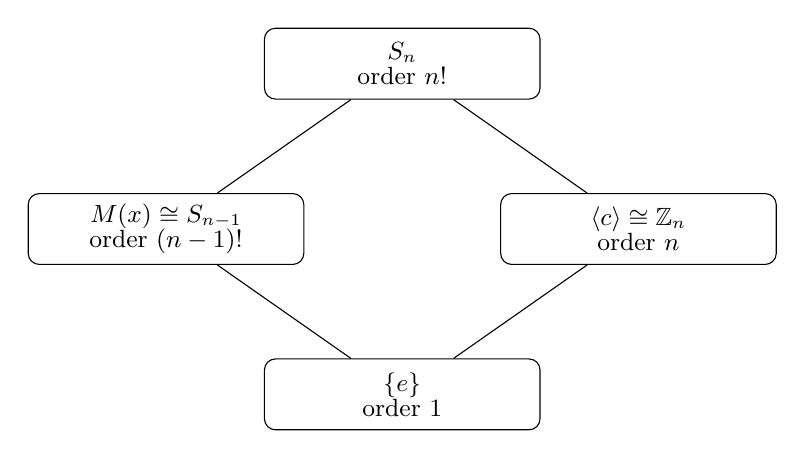
\begin{tikzpicture}[
    node distance=2cm,
    every node/.style={
        draw, rounded corners,
        minimum width=3.5cm,
        minimum height=0.9cm,
        align=center, font=\small
    }
]
\node (Sn)   at (0,   4.2) {$S_n$\\[-2pt]order $n!$};
\node (stab) at (-3,  2.1) {$M(x) \cong S_{n-1}$\\[-2pt]order $(n-1)!$};
\node (cyc)  at ( 3,  2.1) {$\langle c \rangle \cong \mathbb{Z}_n$\\[-2pt]order $n$};
\node (e)    at (0,   0)   {$\{e\}$\\[-2pt]order $1$};
\draw (Sn) -- (stab);
\draw (Sn) -- (cyc);
\draw (stab) -- (e);
\draw (cyc)  -- (e);
\end{tikzpicture}
\caption{Subgroup lattice (Hasse diagram). An edge from $A$ to $B$ with
$A$ below $B$ denotes $A \leq B$. $M(x)$ and $\langle c \rangle$ are
incomparable for $n \geq 3$.}
\label{fig:lattice}
\end{figure}

\subsection{Incomparability of $M(x)$ and $\langle c \rangle$}

\begin{proposition}
For $n \geq 3$, $M(x)$ and $\langle c \rangle$ are incomparable subgroups
of $S_n$, and $M(x) \cap \langle c \rangle = \{e\}$.
\end{proposition}

\begin{proof}
For $n = 3$, $x = 1$: $M(1) = \{e,(2\ 3)\}$ and
$\langle c \rangle = \{e,(1\ 2\ 3),(1\ 3\ 2)\}$.
The transposition $(2\ 3)$ fixes $1$, so $(2\ 3) \in M(1)$, but it is
not a power of $(1\ 2\ 3)$, so $(2\ 3) \notin \langle c \rangle$.
The element $(1\ 2\ 3)$ satisfies $(1\ 2\ 3)(1) = 2 \neq 1$, so
$(1\ 2\ 3) \notin M(1)$. The subgroups are therefore incomparable, and
$M(1) \cap \langle c \rangle = \{e\}$.

For $n > 3$: $M(x)$ always contains transpositions $(y\ z)$ with
$y, z \neq x$, which have order $2$. Non-identity elements of
$\langle c \rangle$ have order dividing $n$ with no order-$2$ element
when $n$ is odd; for even $n$ one verifies directly that order-$2$ powers
of $c$ do not fix $x$. The incomparability holds in all cases.
\end{proof}

\noindent\textbf{OS interpretation.} For $n \geq 3$, the mutex-admissible
schedules and the round-robin schedules are almost entirely disjoint.
Imposing both constraints simultaneously leaves only $e$ --- the deadlock
state under Assumption~\ref{ass:deadlock}. This reflects a structural
separation between the safety constraint (mutex) and the fairness constraint
(round-robin) within the scheduling space.

\subsection{Limitations}

\begin{itemize}
    \item \textbf{Single epoch.} Dynamic properties such as liveness or
          starvation freedom require sequences of epochs, which $S_n$
          does not model.
    \item \textbf{Deadlock modeling.} Assumption~\ref{ass:deadlock} is an
          operational identification, not a derivation from Coffman
          conditions. A fuller treatment would require a group-theoretic
          model of the resource allocation graph.
    \item \textbf{Single critical slot.} Multi-resource mutex requires
          computing $\bigcap_i \mathrm{Stab}(x_i)$, which is a valid
          subgroup but is not developed here.
\end{itemize}

\subsection{Possible Extensions}
\label{sec:extensions}

\begin{itemize}[noitemsep]
    \item Multi-resource mutex as $\bigcap_i \mathrm{Stab}(x_i)$
    \item Readers-writers as a double coset decomposition
    \item Scheduling histories as paths in the Cayley graph of $S_n$
    \item Deadlock detection via a group-theoretic model of the
          resource allocation graph
\end{itemize}

% -----------------------------------------------------------------------
\section{Conclusion}
% -----------------------------------------------------------------------

We have formalized three OS synchronization mechanisms as subgroup-theoretic
restrictions on $S_n$, within the epoch-based model of
Section~\ref{sec:assumptions}, and verified them computationally for
$n \leq 6$:

\begin{enumerate}
    \item The unrestricted scheduling space is $S_n$ with $n!$ elements.
    \item Mutual exclusion corresponds to the stabilizer subgroup
          $M(x) \cong S_{n-1}$ of order $(n-1)!$, with $n$ left cosets
          partitioning the scheduling space into one admissible region
          and $n-1$ violation regions.
    \item Round-robin scheduling corresponds to the cyclic subgroup
          $\langle c \rangle \cong \mathbb{Z}_n$ of order $n$, which is
          transitive (starvation-free), abelian, and not normal in $S_n$
          for $n \geq 3$.
    \item Under Assumption~\ref{ass:deadlock}, deadlock corresponds to
          the identity element $e$ --- the unique permutation under which
          no process advances.
\end{enumerate}

The subgroups $M(x)$ and $\langle c \rangle$ are incomparable for
$n \geq 3$, meeting only at $\{e\}$. This reflects a structural separation
between the safety and fairness constraints in the scheduling space.
Source code and notebooks are available at \cite{repo}.

% -----------------------------------------------------------------------
\begin{thebibliography}{9}

\bibitem{silberschatz}
    A.~Silberschatz and P.~B.~Galvin,
    \textit{Operating System Concepts},
    International Student Version, 8th~ed.
    Wiley India, 2010.

\bibitem{gallian}
    J.~A.~Gallian,
    \textit{Contemporary Abstract Algebra}, 8th~ed.
    Cengage Learning, 2017.

\bibitem{coffman}
    E.~G.~Coffman, M.~J.~Elphick, and A.~Shoshani,
    ``System Deadlocks,''
    \textit{ACM Computing Surveys},
    vol.~3, no.~2, pp.~67--78, 1971.

\bibitem{claude}
    Anthropic,
    \textit{Claude} (AI assistant, Claude Sonnet 4.6).
    \url{https://www.anthropic.com}, 2026.
    Used for code generation, notebook structure, and manuscript drafting.

\bibitem{repo}
    O.~P.~Mohanty,
    \textit{OS Symmetry Synchronization --- Source Code and Notebooks},
    GitHub, 2026.
    \url{https://github.com/04pranab/os-symmetry-synchronization}

\end{thebibliography}

\end{document}